\subsection{Formalization}
\label{sec:formalization}

Let $S$ be a set of stable bug fixing patches and $P$ a set of all bug fixing patches in Linux kernel. We call $U \in (S \cap P ) $ is a set of unknown bug fixing. In our problem, we try to provide a bug fixing patches ranking $\subset P^2$ for a developer, where each bug fixing patch has to meet the following properties~\cite{rendle2009bpr}:
\begin{itemize}
	\item \textit{Totality:} $\forall i,j \in P: i \neq j \Rightarrow (i > j) \vee (j > i)$
	\item \textit{Antisymmetry:} $\forall i,j \in P: (i > j) \wedge (j > i) \Rightarrow i = j$ 
	\item \textit{Transitivity:} $\forall i,j,k \in P: (i > j) \vee (j > k) \Rightarrow i > k$ 
\end{itemize}

\subsection{Bug Fixing Patch Ranking}
\label{sec:bugranking}
\begin{figure*}[t!]
	\centering
	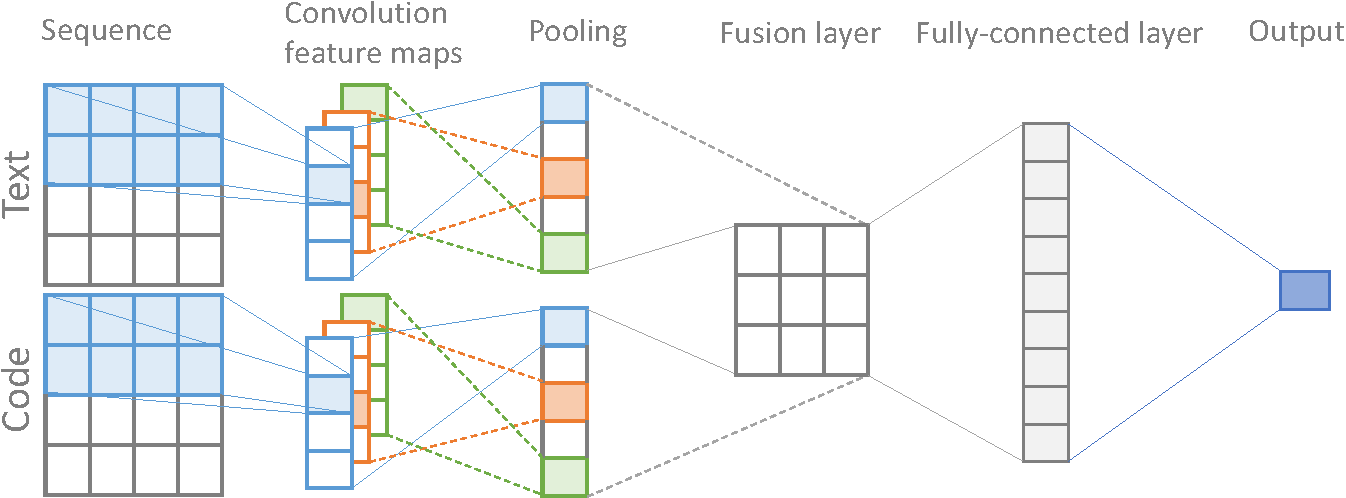
\includegraphics[width=1.0\textwidth]{BugPatchingRanking_v4-cropped.pdf}
	\caption{An architecture of bug fixing patches ranking model in Linux kernel.}
	\label{fig:bugranking}
\end{figure*}

The architecture of bug fixing patch ranking is represented in Fig.~\ref{fig:bugranking}. Our model based on convolutional neural network~\cite{lecun1995convolutional} to map bug fixing patches to vectors, which can be used to compute their ranking score. In the following, we describe how the model computes the ranking score given by a pair of bug fixing patches. We briefly explain each component (i.e., hidden layer, logistic function, etc.) of our model.

\subsection{Learning Relationship Between Text and Code in Single Patch}
\label{sec:learningTextandCode}
In Linux kernel, each patch contains both a textual commit message and commit code. The commit message, which can help a developer to speed up the reviewing process, is a short description of source code change. The commit code is the changes that are applied on the buggy file. 